\documentclass{beamer}
%Arquivo com os principais pacotes usados e suas descrições.

%%%%%%%%%%%%%%%%%%%%%%%%%%%%%%%%%%%%%%%%%
% 			Idiomas e Acentos			%
%%%%%%%%%%%%%%%%%%%%%%%%%%%%%%%%%%%%%%%%%
\usepackage[brazil]{babel} % Habilita o uso do idioma português do brasil (PT-BR).
\usepackage[T1]{fontenc} 
%\usepackage{fontspec} % Habilita maior variedade de acentos. Pode ser necessario adicionar outros pacotes.
\usepackage{lmodern} % Habilita o uso da font Latin Modern.


%%%%%%%%%%%%%%%%%%%%%%%%%%%%%%%%%%%%%%%%%
% 				TABELAS					%
%%%%%%%%%%%%%%%%%%%%%%%%%%%%%%%%%%%%%%%%%
\usepackage{tabulary} % Cria tabelas mais facilmente.
\usepackage{booktabs} % Melhora o visual das tabelas.

%\usepackage[table]{xcolor} % Pacote de cor pra as tabelas.

\usepackage{caption} % Melhora as legendas de imagens, tabela etc.

%%%%%%%%%%%%%%%%%%%%%%%%%%%%%%%%%%%%%%%%%
% 				IMAGENS					%
%%%%%%%%%%%%%%%%%%%%%%%%%%%%%%%%%%%%%%%%%
%\usepackage{graphicx} % Facilita a inserção de imagens.


%%%%%%%%%%%%%%%%%%%%%%%%%%%%%%%%%%%%%%%%%
% 			CÓDIGO FONTE				%
%%%%%%%%%%%%%%%%%%%%%%%%%%%%%%%%%%%%%%%%%
%Documentação de código fonte.
\usepackage{listings}


%%%%%%%%%%%%%%%%%%%%%%%%%%%%%%%%%%%%%%%%%
% 	Símbolos e Caracteres Matemáticos	%
%%%%%%%%%%%%%%%%%%%%%%%%%%%%%%%%%%%%%%%%%
\usepackage{amsmath}
\usepackage{amssymb}
\usepackage{amsfonts}
%\usepackage{mathspec} %Habilita o uso das fontes e dos caracteres matematicos.


%%%%%%%%%%%%%%%%%%%%%%%%%%%%%%%%%%%%%%%%%
%				ABNT					%
%%%%%%%%%%%%%%%%%%%%%%%%%%%%%%%%%%%%%%%%%
%\usepackage[alf]{abntcite} % Ordena as referencias em ordem alfabética.
\usepackage{url} %Facilita o uso de url. Pode-se usar o comando \url{...}.


%%%%%%%%%%%%%%%%%%%%%%%%%%%%%%%%%%%%%%%%%
% 			Configurações				%
%%%%%%%%%%%%%%%%%%%%%%%%%%%%%%%%%%%%%%%%%
\captionsetup{justification=centering,labelfont=bf} %Formata a legenda das figuras.
%\graphicspath{{../imgs/}} %Define o diretorio padrão para buscar as imagens da apresentação.  
%\setromanfont[Ligatures=TeX]{Crimson}
%\defaultfontfeatures{Scale=MatchLowercase, Mapping=tex-tex}

%%%%%%%%%%%%%%%%%%%%%%%%%%%%%%%%%%%%%%%%%
%				BEAMER					%
%%%%%%%%%%%%%%%%%%%%%%%%%%%%%%%%%%%%%%%%%
%Define algumas configurações que serão validas para todo o documento.  
\setbeamertemplate{section in toc}[sections numbered]
\setbeamertemplate{subsection in toc}[subsections numbered]
\setbeamertemplate{background canvas}[vertical shading][bottom=blue!3,top=blue!7]
\setbeamertemplate{caption}[numbered]

\PassOptionsToPackage{table}{xcolor}
\usetheme{Berlin}

\author{Guilherme A. de Macedo \\
        Victor H. Carlquist da Silva
}

\title{Agile Modeling}
\date{\today}

\begin{document}

    \frame{
        \titlepage
    }
	
	%victor
	\frame{\frametitle {Introdução}
	    \begin{itemize}
	        \item Modelar e documentar \textit{software};
	        \item Coleção de valores, princípios e práticas;
	        \item Desenvolver os processos com confiança;
	        \item É combinado com outras técnicas (Scrum, XP, etc...)
	    \end{itemize}
	}
	%Guilherme
	\frame{\frametitle {Desenvolvimento Dirigido ao Modelo Ágil}
	    \begin{itemize}
	        \item Desenvolvimento Dirigido a Modelos;
	        \item Desenvolvimento Dirigido ao Modelo Ágil.
	    \end{itemize}
	}
	%victor
	\frame{\frametitle {Melhores práticas da Modelagem Ágil}
	    \begin{enumerate}
	        \item Outubro de 2000 começou a definição dos valores, princípios e práticas.
	        \item Definição muito específica dos passos, difícil de entender;
	        \item Em 2003 - Agile Model Driven Development (AMDD) (práticas).
	    \end{enumerate}
	}
	%Guilherme
	\frame{\frametitle {Valores da Modelagem Ágil}
	    \begin{itemize}
	        \item Quatro valores herdados da Extreme Programming (Ken Beck):
                \begin{enumerate}
                    \item Comunicação - Modelos promovem a comunicação;
                    \item Simplicidade - É mais fácil entender diagramas do que linhas de códigos;
                    \item Feedback - Comunicar ideias através de diagramas gera feedback mais rápido;
                    \item Coragem - Para tomar importantes decisões e mudar a direção caso alguma decisão tomada se mostre inadequada.
                \end{enumerate}
            \item Humildade/Respeito - Os melhores desenvolvedores sabem que não sabem tudo.
            \begin{itemize}
                \item Huet Landry sugeriu o conceito de "Outra-Estima" em detrimento da "Auto-Estima".
            \end{itemize}
	    \end{itemize}
	}
	
	%victor
	%
	%
	%
	%
	%
	%portoimagem.wordpress.com
	%
	%
	\frame{\frametitle {Princípios da Modelagem Ágil}
	    \begin{itemize}
	        \item Modelagem Ágil possuí 11 princípios principais;
	    \end{itemize}
	}
	%victor
	\frame{\frametitle {Princípios da Modelagem Ágil}
	\begin{figure}
		\caption{Modele com um propósito}
	        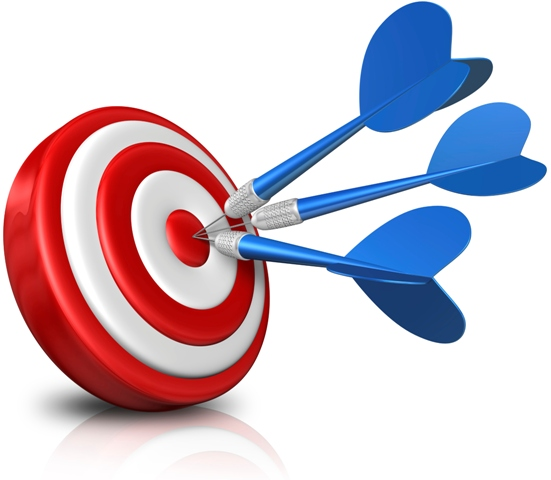
\includegraphics[width = 7cm,keepaspectratio]{img/alvo}
	    \caption*{fonte: coracoesabrasados.blogspot.com}
	    \end{figure}
	}
	%victor
	\frame{\frametitle {Princípios da Modelagem Ágil}
	\begin{figure}
		\caption{Maximizar os investimentos dos Stakeholder}
	        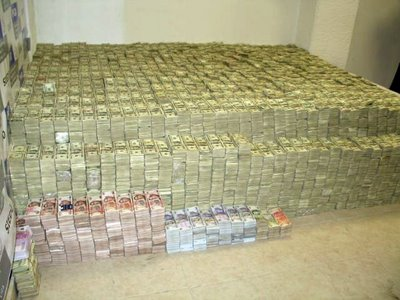
\includegraphics[width = 7cm,keepaspectratio]{img/invetimento}
	    \caption*{fonte: blogdaprata-pb.blogspot.com}
	    \end{figure}
	}
	%victor
	\frame{\frametitle {Princípios da Modelagem Ágil}
	\begin{figure}
		\caption{Viajar leve}
	        
\includegraphics[width = 7cm,keepaspectratio]{img/viajar}
	    \caption*{fonte: www.dailytech.com}
	    \end{figure}
	}
	%victor
	\frame{\frametitle {Princípios da Modelagem Ágil}
	\begin{figure}
		\caption{Multiplos modelos}
	        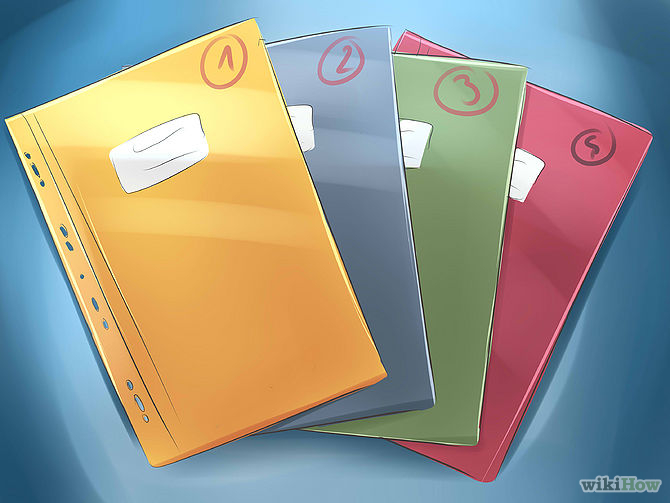
\includegraphics[width = 7cm,keepaspectratio]{img/modelos}
	    \caption*{fonte: www.wikihow.com}
	    \end{figure}
	}
	%victor
	\frame{\frametitle {Princípios da Modelagem Ágil}
	\begin{figure}
		\caption{Feedback rápido}
	        
\includegraphics[width = 7cm,keepaspectratio]{img/feedback}
	    \caption*{fonte: beatriziolanda.com}
	    \end{figure}
	}
	%victor
	\frame{\frametitle {Princípios da Modelagem Ágil}
	\begin{figure}
		\caption{Ser simples}
	        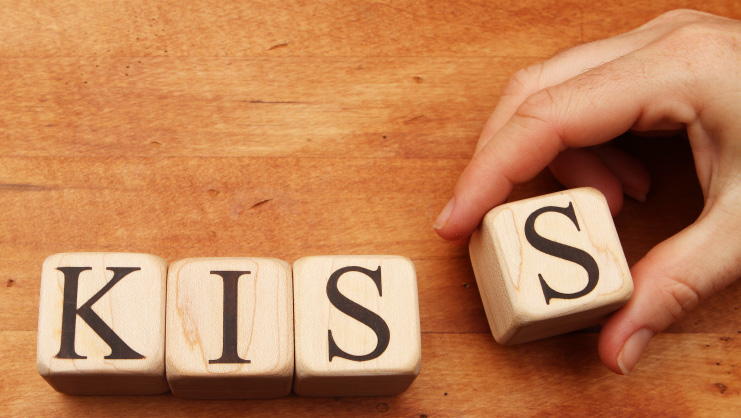
\includegraphics[width = 7cm,keepaspectratio]{img/kiss}
	    \caption*{fonte: reginagiannetti.wordpress.com}
	    \end{figure}
	}
	%victor
	\frame{\frametitle {Princípios da Modelagem Ágil}
	\begin{figure}
		\caption{Aceite Mudanças}
	        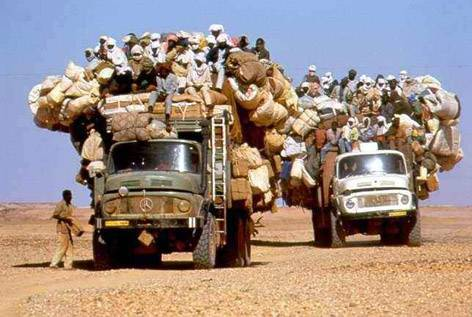
\includegraphics[width = 7cm,keepaspectratio]{img/mudanca}
	    \caption*{fonte: suzyqscraps.com}
	    \end{figure}
	}
	%victor
	\frame{\frametitle {Princípios da Modelagem Ágil}
	\begin{figure}
		\caption{Mudança incremental}
	        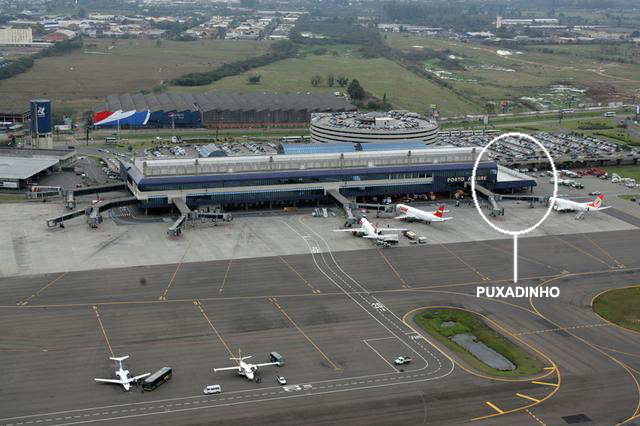
\includegraphics[width = 7cm,keepaspectratio]{img/incremental}
	    \caption*{fonte: pitacoazul.blogspot.com}
	    \end{figure}
	}
	%victor
	\frame{\frametitle {Princípios da Modelagem Ágil}
	\begin{figure}
		\caption{Trabalho de qualidade}
	        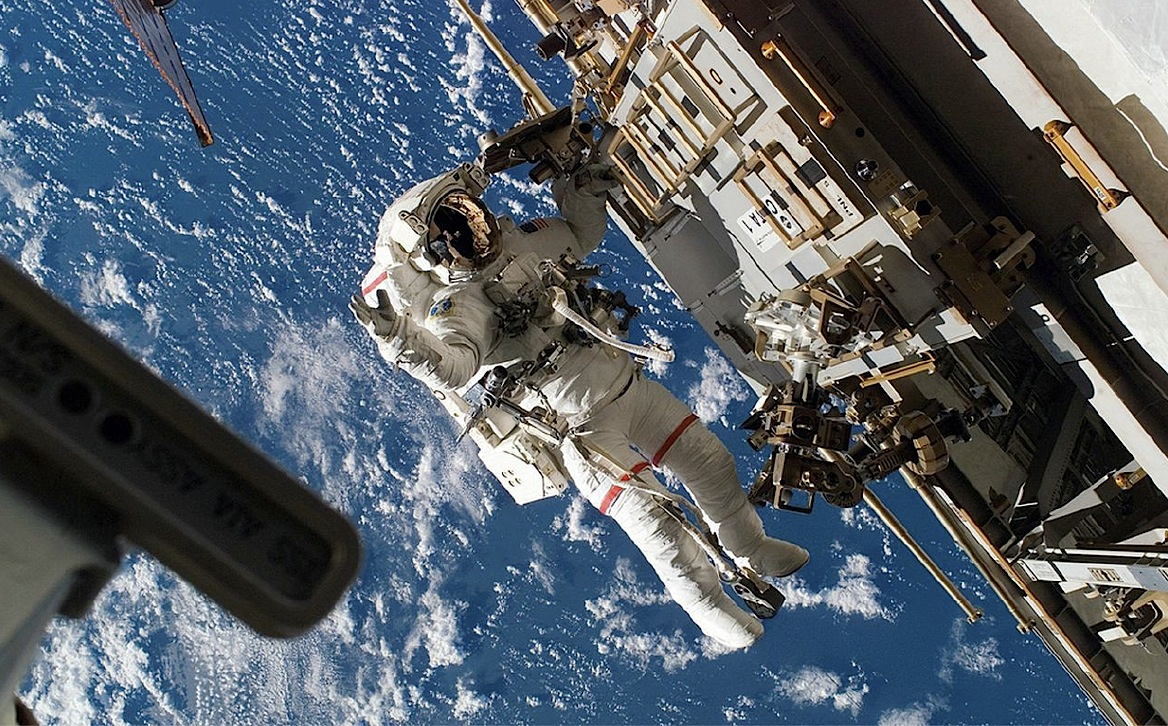
\includegraphics[width = 7cm,keepaspectratio]{img/iss}
	    \caption*{fonte: portoimagem.wordpress.com}
	    \end{figure}
	}
	%victor
	\frame{\frametitle {Princípios da Modelagem Ágil}
	\begin{figure}
		\caption{Software funcional é o objetivo primário}
	        
\includegraphics[width = 7cm,keepaspectratio]{img/software}
	    \caption*{fonte: www.profissionaisti.com.br}
	    \end{figure}
	}
	%victor
	\frame{\frametitle {Princípios da Modelagem Ágil}
	\begin{figure}
		\caption{Outros recursos é o objetivo secundário}
	        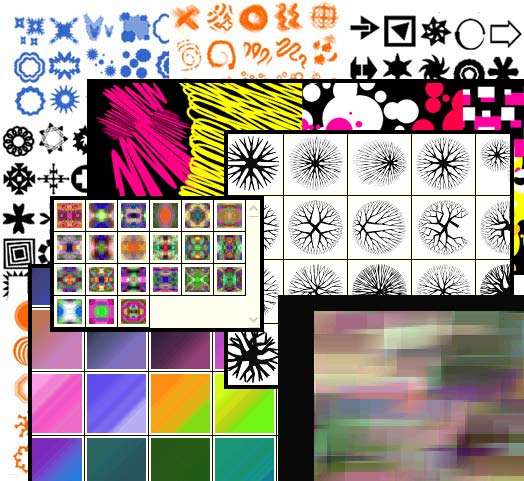
\includegraphics[width = 7cm,keepaspectratio]{img/recur}
	    \caption*{fonte: forum.imasters.com.br}
	    \end{figure}
	}
	
	%Guilherme
	\frame{\frametitle {Práticas da Modelagem Ágil}
	    \begin{itemize}
	        \item 13 - Principais:
	        \item 5 - Suplementares:
	    \end{itemize}
	}

	%Guilherme
	\frame{\frametitle {Práticas da Modelagem Ágil - Principais}
	    \begin{enumerate}
	        \item Participação ativa dos envolvidos; \pause
	        \item Não modele sozinho; \pause
	        \item Aplique os artefatos corretamente; \pause
	        \item Itere para outro artefato; \pause
	        \item Prove a modelagem com código; \pause
	        \item Use ferramentas simples; \pause
	        \item Modele utilizando incrementos pequenos; \pause
	        \item Armazene as informações em apenas um lugar; \pause
	        \item Propriedade coletiva; \pause
	        \item Trabalhe com vários modelos em paralelo; \pause
	        \item Crie conteúdo simples; \pause
	        \item Utilize apenas modelos descritivos; \pause
	        \item Exponha os modelos publicamente.
	    \end{enumerate}
	}
	
	%Guilherme
	\frame{\frametitle {Práticas da Modelagem Ágil - Suplementares}
	    \begin{enumerate}
	        \item Aplique padrões de modelagem; \pause
	        \item Tenha cuidado ao aplicar padrões; \pause
	        \item Descarte modelos temporários; \pause
	        \item Formalize os modelos de contrato; \pause
	        \item Atualize somente quando for necessário.
	    \end{enumerate}
	}	
	
	% Guilherme 
	\frame{\frametitle {Críticas à Modelagem Ágil}
	    \begin{itemize}
	        \item Requer desenvolvedores de nível sênior;
	        \item Requer mudança cultural;
	        \item Pode levar a maiores dificuldades nas negociações contratuais.
	    \end{itemize}
	}
	
	% Victor
	\frame{\frametitle {Conclusão}
	    \begin{itemize}
	        \item Quando utilizar e quando não utilizar a Modelagem Ágil?
	    \end{itemize}
	}
\end{document}
		
